\chapter{Propuesta solución: Aplicación Aprende Fácil}
\label{cap:aprendeFacil}



%-------------------------------------------------------------------
\section{Diseño centrado en el usuario de los prototipos de la Aplicación}
%-------------------------------------------------------------------
\label{cap:sec:disenioInterfaz}
Como ya se ha explicado en capítulos anteriores, esta aplicación está creada por y para personas que tienen alguna discapacidad cognitiva, por lo que el diseño de la interfaz debe ser sencillo y su uso no debe llevar a confusión ni debe hacer sentir al usuario frustrado al usarla. 
Es por ello que el diseño debe estar centrado en el usuario, y en nuestro caso aún más puesto que los usuarios finales requieren un diseño centrado en sus necesidades. Así pues, al ser un campo poco conocido por lo integrantes del equipo, se ha necesitado de la ayuda de expertos para saber con mas detalle cual es el diseño adecuado. 
El diseño de la aplicación se ha realizado en dos iteraciones: una iteración competitiva entre los integrantes del grupo y una segunda iteración con expertos del Colegio Estudio3 Afanias\footnote{https://afanias.org/que-hacemos/educacion/colegio-estudio-3/}. 

%-------------------------------------------------------------------
\subsection{Primera Iteración: Iteración Competitiva}
%-------------------------------------------------------------------
\label{cap:subsec:iteracionCompetitiva}

En esta primera iteración cada integrante del grupo ha realizado su propio diseño de la aplicación. En la realización de estos diseños, los integrantes no podían hablar entre ellos ni comentar las diferentes ideas que tenían para la implementación. De esta forma se consigue que los diseños sean totalmente dispares y que las ideas de uno no provoquen la modificación del diseño del otro y que surjan ideas distintas.
Se realizaron cuatro prototipos distintos ya que no teníamos claro si los usuarios finales iban a preferir que se mostrara un solo significado o todos, si mostrar la definición y el ejemplo les iba a ayudar o no y si añadir los pictogramas les ayudaría o no.
Los prototipos fueron los siguientes:
\begin{itemize}
	\item Prototipo 1: Se muestra un único significado, siendo este el más común e incluyendo las comparaciones.
	\item Prototipo 2: Se muestra el significado más común, junto con una definición tradicional del concepto e incluyendo las comparaciones.
	\item Prototipo 3: Se muestran todos los significados de la palabra buscada e incluyendo las comparaciones.
	\item Prototipo 4: Se muestran todos los significados de la palabra y se añaden pictogramas\footnote{Se entiende como pictograma un dibujo, imagen o figura que representa el significado de una palabra.} a las palabras, haciendo así que la comprensión del concepto sea mucho mas sencilla. Tanto en el prototipo diseñado por Pablo como en el de Irene se han utilizado los pictogramas de ARASAAC\footnote{http://www.arasaac.org/}.
	
\end{itemize}

En las Figuras \ref{fig:mockup1pablo}, \ref{fig:mockup2pablo}, \ref{fig:mockup3pablo} y \ref{fig:mockup4pablo} se muestran los prototipos creados por Pablo y en las Figuras \ref{fig:mockup1irene_vInicial}, \ref{fig:mockup2irene_vInicial},  \ref{fig:mockup3irene_vInicial} y \ref{fig:mockup4irene_vInicial} los prototipos creados por Irene.

Una vez que los prototipos estaban terminados, lnos juntamos para hacer una puesta en común y analizar los prototipos creados. 
Por lo general, los prototipos de los dos integrantes del grupo eran bastantes similares, las principales diferencias eran:

\begin{itemize}
	\item Ambos prototipos integran los mismos elementos: un campo de texto para introducir la palabra, un botón de búsqueda y los resultados se muestran en forma de lista, agrupando los distintos resultados en rectángulos, que a partir de ahora denominaremos fichas.
	Pablo ha optado por formas rectangulares, tanto para las fichas como para el campo de texto, mientras que Irene utiliza formas redondeadas en todos los elementos. 
	Por otro lado, Pablo implementó un diseño orientado a niños por lo que para el color utilizó azules muy suaves y fondos juveniles con lápices de colores, gomas de borrar, etc.  Irene utilizó un color mostaza, siendo un diseño más simple pero intentando abarcar a un usuario de cualquier edad. Por último, los resultados del prototipo de Irene, se muestran en color mostaza indicando de esta forma que se pueden pinchar en ellos, y se realizará la búsqueda del concepto pulsado.
	
	\item El orden a la hora de mostrar los resultados es distinto. En los prototipos de Pablo se muestran primero las metáforas (\textit{Un vehículo es una máquina} o \textit{Un vehículo es un transporte}), después los símiles (\textit{Un vehículo es como un taxi}) y finalmente las analogías (\textit{Un vehículo es rápido como un caballo}). En los prototipos de Irene se muestra únicamente una analogía, una metáfora y un símil para cada significado de la palabra buscada.
	
	\item En el prototipo 3 de Pablo incluye justo debajo de los resultados mostrados un ejemplo siempre visible (``Él necesita un coche para ir a trabajar'') para facilitar al usuario la comprensión del término buscado.
	
	 \item En el prototipo 3 de Irene incluye justo debajo de los resultados mostrados una definición dentro de un botón (``Vehículo motorizado de cuatro ruedas por lo general impulsado por un motor de combustión interna'') dando a elegir al usuario la decisión de poder verla o no.
	
	\item Pablo decidió añadir el título ``Un X es ...'' antes de la lista de los resultados, englobando de esta forma los conceptos que tienen el mismo significado. Si existen varias acepciones del concepto, añade el título ``O también puede ser...'' en los siguientes, dejando claramente divididos los distintos significados que pudieran existir para el concepto buscado. En cambio Irene, añade un único título al principio (``Resultados para la palabra X'') donde queda claro que los resultados que se obtienen son para dicho concepto y además añade delante de cada metáfora: ``Un X es...''  y delante de cada símil y analogía: ``Un X es como...''.

	\item Para la numeración de los resultados obtenidos, Pablo incluye dentro de cada ficha un listado numérico e Irene únicamente añade un número a la ficha.
	
	\item En el prototipo donde se incluyen también los pictogramas, Pablo añade un pictograma que hace referencia al concepto buscado según el contexto en que se utilice. Por ejemplo, un vehículo puede hacer referencia a un coche o puede ser un medio para llegar o lograr un fin, por lo que el añade el pictograma en función de su significado, e Irene además de incluir el mismo pictograma que Pablo, añade pictogramas a las palabras usadas en las comparaciones. Por ejemplo, en la frase ``Un portero es un vigilante'' Irene añadió el pictograma de vigilante.
\end{itemize}



Una vez analizados los prototipos de ambos integrantes nos reunimos con los directores del trabajo y se decidió crear un prototipo con las siguientes características:


\begin{itemize}
	\item Para el diseño de la interfaz se eligió el de Irene por tener una interfaz más atractiva.
	\item Se eligió la palabra Portero para utilizarla como ejemplo en todos los prototipos.
	\item El orden de las resultados se modificó, haciendo que primero aparezcan las metáforas (``Un portero es un vigilante''), después los símiles (``Un portero es como un guardia'') y por último las analogías  (``Un portero es tan ágil como un pájaro'').
	\item Se eliminó la palabra \textit{tan} en la plantilla usada para las analogías.
	\item Se creó un nombre para la aplicación que estuviese en español: ``Aprende Fácil''.
	\item En vez de mostrar un único símil, una metáfora y una analogía. Se deben mostrar todos los resultados obtenidos para dicho concepto.
	\item Se decidió que si la palabra solo tenía un significado se eliminaba el número de la ficha.
	\item Se añadió un pictograma a la característica que relaciona el concepto con el resultado en las analogías. Por ejemplo, en la frase \textit{Un portero es tan fuerte como un gorila}  se añadió el pictograma correspondiente a fuerte.
	\item Dejar el ejemplo del prototipo de Pablo junto con la definición del prototipo de Irene.
	\item Crear un nuevo prototipo donde la definición y el ejemplo se muestren a primera vista, y el usuario no tenga que estar pinchando en ningún botón para que los expertos nos indiquen cual es la mejor opción.
	\item Crear otro prototipo donde la definición y el ejemplo estén separados. Así el usuario puede elegir lo que quiere ver, si solo una cosa o ambas.
\end{itemize} 

Con todas estas decisiones, se crearon los prototipos que se muestran en las Figuras \ref{fig:mockup1irene_vFinal}, \ref{fig:mockup2irene_v1_vFinal}, \ref{fig:mockup2irene_v2_vFinal}, \ref{fig:mockup2irene_v3_vFinal}, \ref{fig:mockup3irene_vFinal}, \ref{fig:mockup4irene_vFinal} y que fueron los que se usaron para en la siguiente iteración donde nos reunimos con los expertos para que nos dieran su opinión sobre la aplicación, y nos ayudarán a decidir sobre los siguientes aspectos:
\begin{itemize}
	\item ¿Se debe mostrar el significado más común o todos los significados de la palabra buscada?
	\item ¿Se debe añadir la definición tradicional y el ejemplo junto con las figuras retóricas o no?  Y en caso de añadirlos, ¿Se deben mostrar juntos en un mismo botón, en distintos botones o sin botón y que aparezcan debajo de los resultados?
	\item ¿Son útiles los pictogramas? En caso de serlo, ¿solamente el pictograma de la palabra buscada o también añadimos los pictogramas de las palabras que se usan en las figuras retóricas?
	\item ¿La forma de mostrar los resultados es correcta, o es mejor otra disposición?
	
\end{itemize} 


 	\figura{Bitmap/Mockups/mockup1_pablo}{width=1.0\textwidth}{fig:mockup1pablo}{Prototipo de Pablo mostrando resultado más común para la palabra vehículo}
	\figura{Bitmap/Mockups/mockup2_pablo}{width=.9\textwidth}{fig:mockup2pablo}{Prototipo de Pablo mostrando resultado más común para la palabra vehículo y un ejemplo} 
	\figura{Bitmap/Mockups/mockup3_pablo}{width=.9\textwidth}{fig:mockup3pablo}{Prototipo de Pablo mostrando todos los resultados para la palabra vehículo} 
 	\figura{Bitmap/Mockups/mockup4_pablo}{width=.9\textwidth}{fig:mockup4pablo}{Prototipo de Pablo mostrando todos los resultados para la palabra vehículo junto con pictogramas} 
 	
 	\figura{Bitmap/Mockups/mockup1_irene_inicial.png}{width=1.2\textwidth}{fig:mockup1irene_vInicial}{Prototipo de Irene mostrando resultado más común para la palabra vehículo}
 	\figura{Bitmap/Mockups/mockup2_irene_inicial.png}{width=1.2\textwidth}{fig:mockup2irene_vInicial}{Prototipo de Irene mostrando resultado más común para la palabra vehículo y una definición}
	\figura{Bitmap/Mockups/mockup3_irene_inicial.png}{width=1.2\textwidth}{fig:mockup3irene_vInicial}{Prototipo de Irene mostrando todos los resultados para la palabra portero} 
	\figura{Bitmap/Mockups/mockup4_irene_inicial.png}{width=1.2\textwidth}{fig:mockup4irene_vInicial}{Prototipo de Irene mostrando todos los resultados para la palabra portero junto con pictogramas} 
	
	\figura{Bitmap/Mockups/mockup1_irene_final.png}{width=1.2\textwidth}{fig:mockup1irene_vFinal}{Prototipo mostrando resultado más común para la palabra portero}
	\figura{Bitmap/Mockups/mockup2_irene_final_v1.png}{width=1.2\textwidth}{fig:mockup2irene_v1_vFinal}{Prototipo Versión 1 mostrando resultado más común para la palabra portero junto con una definición y un ejemplo separados}
	\figura{Bitmap/Mockups/mockup2_irene_final_v2.png}{width=1.2\textwidth}{fig:mockup2irene_v2_vFinal}{Prototipo Versión 2 mostrando resultado más común para la palabra portero junto con una definición y un ejemplo a simple vista}
	\figura{Bitmap/Mockups/mockup2_irene_final_v3.png}{width=1.2\textwidth}{fig:mockup2irene_v3_vFinal}{Prototipo Versión 3 mostrando resultado más común para la palabra portero junto con una definición y un ejemplo en un mismo botón}
	\figura{Bitmap/Mockups/mockup3_irene_final.png}{width=1.2\textwidth}{fig:mockup3irene_vFinal}{Prototipo mostrando todos los resultados para la palabra portero}
	\figura{Bitmap/Mockups/mockup4_irene_final.png}{width=1.2\textwidth}{fig:mockup4irene_vFinal}{Prototipo mostrando todos los resultados para la palabra portero incluyendo los pictogramas}

	
	 
%-------------------------------------------------------------------
\subsection{Segunda Iteración: Evaluación con Expertos}
%-------------------------------------------------------------------
\label{cap:subsec:evaluacionExpertos}

El día 26 de Marzo de 2019 a las 09:00h nos reunimos con la directora y los profesores del colegio Estudio3 Afanias\footnote{https://afanias.org/que-hacemos/educacion/colegio-estudio-3/} situado en la Comunidad de Madrid. Este colegio atiende a niños y jóvenes con discapacidad intelectual entre los 3 y 21 años de edad.

Lo primero que hicimos fue presentarles la aplicación y mostrarles los prototipos creados al final de la iteración anterior (Figuras \ref{fig:mockup1irene_vFinal}, \ref{fig:mockup2irene_v1_vFinal}, \ref{fig:mockup2irene_v2_vFinal}, \ref{fig:mockup2irene_v3_vFinal}, \ref{fig:mockup3irene_vFinal}, \ref{fig:mockup4irene_vFinal}).
Una vez expuestos los distintos prototipos, nos dieron la enhorabuena y nos hicieron participes de la gran ayuda que supondría esta herramienta. A continuación nos dieron su opinión sobre distintos aspectos que se podrían mejorar:

\begin{itemize} 
	\item Modificar el color amarillo-mostaza de los textos por un color más oscuro que contraste más con el fondo blanco. El color actual es morado oscuro para la barra que contiene el título de la aplicación y un violeta para resaltar los resultados obtenidos, así como para el botón de Definición y Ejemplo.
	\item El tipo de letra debe ser Arial o Script, ya que son las letras con las que los alumnos están familiarizados y las que mejor entienden.
	\item Añadir un reproductor que lea la frase, para hacer la aplicación accesible a aquellas personas que no puedan leer.
	\item Incluir la opción de poder ver un video para complementar la información devuelta por la aplicación.
	\item Los pictogramas deben situarse debajo de la palabra y no al lado, ya que los expertos comentaron que esto puede llevar a confusión a los alumnos pensando que sería otra palabra más para leer. 
	\item Introducción de distintas personalizaciones:
	\begin{itemize}
		\item Búsqueda en tres niveles: sencillo, medio y amplio. El nivel sencillo sería realizando la búsqueda de las palabras fáciles en las 1.000 palabras más usadas de la RAE, el medio en las 5.000 palabras más usadas de la RAE y el amplio en las 10.000 palabras más usadas de la RAE. 
		\item Añadir una opción que permita poner todos los textos en mayúsculas, haciendo la aplicación más accesible para aquellos alumnos que no entienden los textos en minúsculas.
		\item Dejar que el usuario configure si quiere que aparezca la definición y el ejemplo o no.
		\item Dejar que el usuario configure  si aparecen los pictogramas o no.
	\end{itemize}
\end{itemize}

Teniendo en cuenta las observaciones de los expertos se creo el diseño final de la aplicación.



%-------------------------------------------------------------------
\section{Arquitectura de Aprende Fácil}
%-------------------------------------------------------------------
En este apartado se describirá la arquitectura diseñada para la aplicación. En la Figura \ref{fig:diagrama_arquitectura} se puede ver los distintos componentes por los que está formada.

\begin{figure}[!h]
	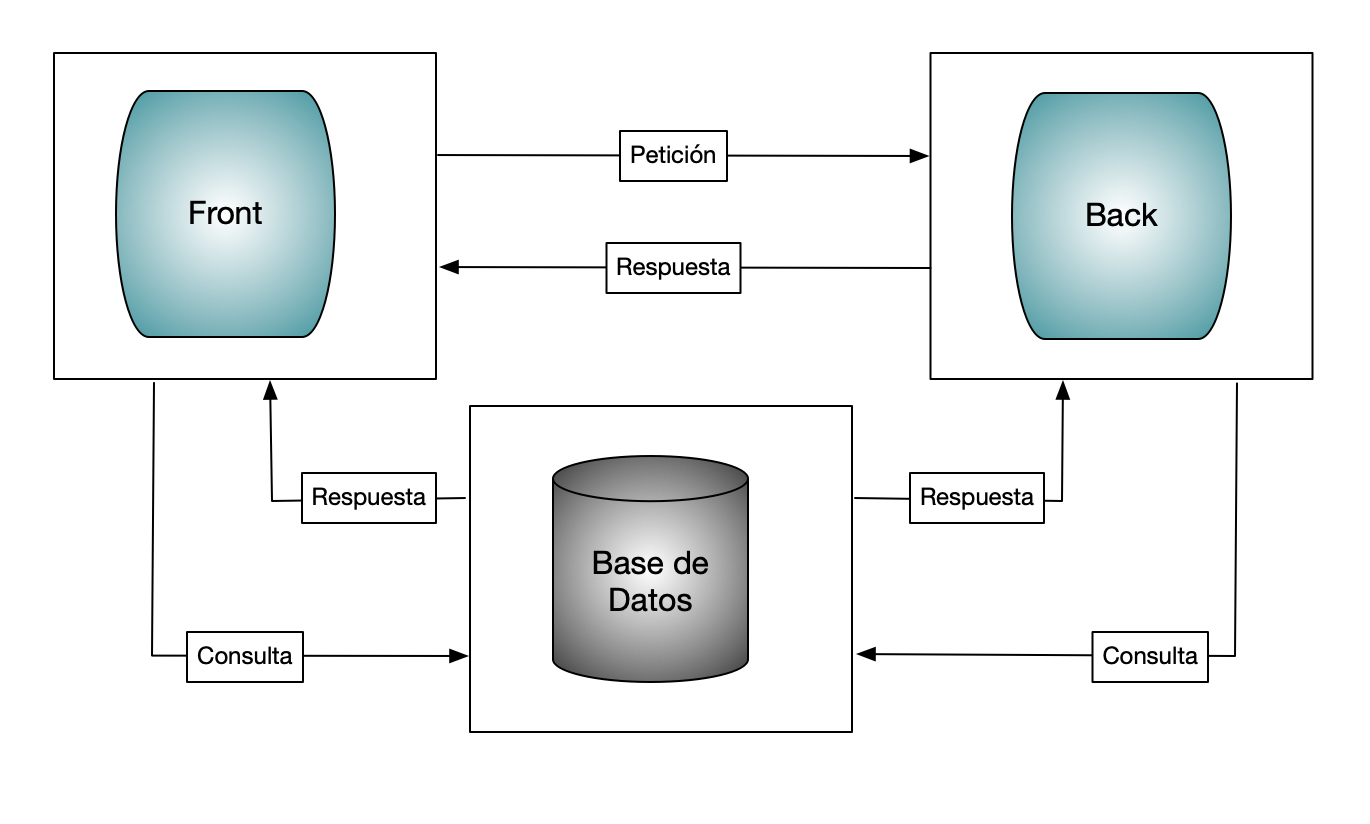
\includegraphics[width=.9\textwidth]{Imagenes/Bitmap/Capitulo4/DiagramaArquitectura.png}
	\caption{Diagrama de la arquitectura del proyecto}
	\label{fig:diagrama_arquitectura}
\end{figure}

La aplicación está formada por una interfaz (\textit{frontend}) la cuál realiza peticiones a la parte interna (\textit{backend}), y este le devuelve la información correspondiente. Para ello, la parte \textit{backend} debe realizar consultas a la base de datos. En la Figura \ref{fig:relacionBackFront}  se puede ver la relación que existe entre el \textit{frontend} con el \textit{backend}, y los servicios web que son utilizados para la obtención de los resultados.
Si el usuario introduce una palabra, dejando por defecto las distintas opciones que vienen y realiza la búsqueda de un concepto, la aplicación invocará a los servicios web relacionados con la obtención de metáforas (\textit{getMetaphor}) y símiles (\textit{getSimil}). A parte, si el usuario seleccionara la opción de ``Mostrar definición y ejemplo'', el servicio web invocado sería el \textit{getDefAndExample} y en caso de seleccionar la opción  ``Mostrar pictos'' se invocaría al servicio web ``getImagen'' para obtener el pictograma del resultado principal y ``getImagenPalabra'' para obtener el pictograma de cada resultado mostrado.

\begin{figure}[!h]
	\includegraphics[width=1.2\textwidth]{Imagenes/Bitmap/Capitulo4/RelacionBackFront.png}
	\caption{Relación entre \textit{Backend} y \textit{Frontend}}
	\label{fig:relacionBackFront}
\end{figure}


 Igualmente en los siguientes apartados se explicará con mayor detalle tanto la implementación del \textit{frontend} como del \textit{backend} . 

Por último, la Universidad Complutense de Madrid nos facilitó un contenedor para poder alojar nuestro trabajo, accesible en la dirección \textit{holstein.fdi.ucm.es}. Este servidor no tenía instalado ningún servicio por lo que se tuvo que realizar la instalación de todo lo necesario (python, pyp, git, mysql, etc). Una vez clonada la rama de GitHub donde tenemos el proyecto, el siguiente paso fue dejar el servidor siempre activo, para ello se tuvo que crear un servicio (\textit{.servi ce}) donde se guardaría la ruta del proyecto.

%-------------------------------------------------------------------
\section{Diseño de la Base de datos de Aprende Fácil}
%-------------------------------------------------------------------



%-------------------------------------------------------------------
\section{Diseño del Backend de Aprende Fácil}
%-------------------------------------------------------------------

%-------------------------------------------------------------------
\subsection{Selección de la Red Semántica a utilizar}
%-------------------------------------------------------------------
\label{cap:subsec:redsemanticautilizada}

En este trabajo necesitamos una herramienta que nos proporcione las palabras relacionadas con un concepto dado y para ello vamos a emplear una red semántica.
Como se ha comentado en el capítulo 2 existen varias redes semánticas que facilitan sinónimos, términos relacionados, metáforas, hiperónimos, etc. de un concepto dado. 
De todas las posibilidades presentadas en la sección 2.1 solo hay dos redes semánticas disponibles para el castellano: WordNet y ConcepNet. Para decidir con cual de las dos quedarnos hicimos una evaluación de ambas para evaluar si los conceptos devueltos por cada herramienta son correctos y sirven para nuestro propósito. En la sección 4.4.1.1 se explicará el diseño de la prueba que se ha realizado para ver que red semántica se utilizará finalmente en el proyecto, en la sección 5.2 se analizarán los resultados cuantitativos de la prueba realizada, en el punto 5.3, se analizarán los resultados obtenidos a nivel cualitativo y en el 5.4 se describirán las conclusiones finales de la evaluación. Por otra parte, en los apartados posteriores, se detallarán los distintos servicios web utilizados para este proyecto, en la sección 5.5 se hablará de la base de datos utilizada y de su estructura, en los apartados 5.6, 5.7 y 5.8 se describirán los servicios web que se utilizan para la obtención de sinónimos, hipónimos e hiperónimos fáciles respectivamente. Por último, se hablará en los puntos 5.9 y 5.10 sobre los servicios web utilizados para crear las metáforas y los símiles que finalmente leerá el usuario.


%-------------------------------------------------------------------
\subsubsection{Diseño de la evaluación}
%-------------------------------------------------------------------
\label{cap:subsec:disenioeval}


Para decidir que red semántica se iba a usar se decidió hacer una prueba con palabras que fuesen lo más heterogéneas posible, para ello se eligieron tres artículos periodísticos de distintos temas: tecnológico\footnote{https://elpais.com/elpais/2019/04/12/ciencia/1555061040\_073105.html}, deportivo\footnote{https://elpais.com/deportes/2019/04/22/actualidad/1555956020\_022201.html} y político\footnote{https://elpais.com/politica/2019/04/23/actualidad/1556019953\_831941.html}. (Los artículos se pueden ver en el Apéndice \ref{sec:apendiceA} )De los artículos se seleccionaron únicamente los verbos, sustantivos y adjetivos, eliminando las palabras que estuvieran repetidas. Finalmente, quedaron 793 palabras para la realización de la prueba, para cada una de estas palabras se obtuvieron en WordNet y ConceptNet sus sinónimos y términos relacionados (en WordNet se entiende como término relacionado a los hiperónimos e hipónimos).

A continuación se comprobó de manera independiente cuantos de los sinónimos y términos relacionados se encontraban en cada una de las tres listas de palabras fáciles\footnote{listas de 1.000, 5.000 y 10.000 palabras más utilizadas en castellano según la RAE} (análisis cuantitativo). Eligiendo como parámetros: porcentaje de palabras introducidas que no generan ningún resultado, porcentaje de palabras sin términos relacionados, porcentaje de palabras sin sinónimos  y cantidad de palabras generadas por cada red semántica(WordNet y ConceptNet). Por último, se analizó la calidad de las palabras obtenidas por cada una de las redes semánticas en cada una de las listas de palabras fáciles, es decir, si las palabras que generaban tenían una relación aceptable con la palabra origen (análisis cualitativo). Eligiendo en ese caso como parámetros el porcentaje de sinónimos correctos y el porcentaje de términos relacionados correctos.

%-------------------------------------------------------------------
\subsubsection{Resultados cuantitativos}
%-------------------------------------------------------------------
\label{cap:sec:pruebaCuantitativa}
\figura{Bitmap/Capitulo4/tabla_cuantitativa}{width=1.0\textwidth}{fig:tabla_cuantitativa}{Tabla de resultados de la prueba cuantitativa} 

En la Tabla \ref{fig:tabla_cuantitativa} se muestran los resultados de la prueba cuantitativa realizada, como se puede observar, en términos generales, WordNet ofrece mejores resultados que ConceptNet ya que el porcentaje de palabras sin términos relacionados, sinónimos o ambas, es mayor en esta última. En el caso de la primera lista utilizada (1.000 palabras fáciles) ConceptNet no encontró ningún resultado para el 68,2\% de las palabras introducidas mientras que WordNet no encontró nada para el 62,6\%. En el caso de los términos relacionados, ConceptNet no encontró ninguno para el 72,1\% de las palabras, mientras que en el caso de WordNet fue del 47,6\%. Para el porcentaje de palabras sin sinónimos los resultados fueron de  La siguiente lista probada fue la de 5.000 palabras fáciles, ConceptNet ha generado 2.652 sinónimos y términos relacionados, mientras que WordNet ha generado 14.172, casi 7 veces más.



%-------------------------------------------------------------------
\subsubsection{Análisis cualitativo}
%-------------------------------------------------------------------
\label{sssec:pruebaCualitativa}
\figura{Bitmap/Capitulo4/tabla_cualitativa}{width=1.0\textwidth}{fig:tabla_cualitativa}{Tabla de resultados de la prueba cualitativa} 
Para realizar el análisis cualitativo de la
Como se puede observar en la Tabla \ref{fig:tabla_cualitativa}, los resultados son muy parejos para ambas redes semánticas. En el caso de la comparación con la lista de las 1.000 palabras fáciles, los sinónimos encontrado por WordNet son mejores que los de ConceptNet (65,45\% de sinónimos correctos frente a 46,15\%) sin embargo los términos relacionados son mejores en ConceptNet (78,67\%) que en WordNet (73,1\%). Después se hizo la comparación con la lista de 5.000 palabras fáciles, ocurre lo mismo que con la lista anterior, hay más sinónimos correctos en WordNet (55,42\%) que en ConceptNet (55\%) y mejores términos relacionados en ConceptNet (84,17\%) que en WordNet (50,6\%). Por último en las comparaciones realizadas con las 10.000 palabras fáciles los resultados en ambos casos, fueron mejores en WordNet (60,73\% en el caso de los sinónimos y 55,3\% en los términos relacionados) que en ConceptNet (53,03\% y 53,19\% respectivamente).


%-------------------------------------------------------------------
\subsubsection{Conclusiones}
%-------------------------------------------------------------------
\label{sssec:conclusionPruebas}

Pendiente de terminar...

%-------------------------------------------------------------------
\section{Servidor de Base de Datos}
%-------------------------------------------------------------------

Para este proyecto, se ha utilizado una base de datos para la persistencia de los datos. El sistema encargado de la gestión de la base de datos corresponde con MariaDB y esta constituida por varias tablas:
\begin{itemize}
	\item Se ha hecho uso de MCR (\textit{Multilingual Central Repository}), utilizando la versión 3.0. 
	MCR es una base de datos de código abierto que integra distintas versiones de WordNet para seis lenguajes diferentes: Inglés, Español, Catalán, Vasco, Gallego y Portugués. Se ha utilizado principalmente la tabla llamada \textbf{wei\_spa-30\_variant} y \textbf{wei\_spa-30\_relation}. De la tabla \textit{Variant} las columnas con las que hemos trabajado han sido:
	\begin{itemize}
		\item \textit{Word}: Contiene la palabra. De esta forma se pueden realizar búsquedas cuando el usuario introduce el concepto para de esta forma saber si dicha palabra se encuentra en la base de datos.
		\item \textit{Offset}: Es el identificador de la palabra, aunque una misma palabra puede tener distintos \textit{offsets}. Con dicha columna se pueden obtener los sinónimos, así como el identificador para posteriormente obtener los hipónimos e hiperónimos.
	\end{itemize}
	\item Tres tablas llamadas \textbf{1000\_palabras\_faciles}, \textbf{5000\_palabras\_faciles} y \textbf{10000\_palabras\_faciles} que guardan tanto las 1.000, 5.000 y 10.000 palabras más usadas de la RAE. Las tres se componen únicamente de una columna llamada \textit{word} y que almacena la palabra.
	\item Una tabla llamada \textbf{datos\_picto}, que está formada por las siguientes columnas:
	\begin{itemize}
		\item Palabra: Contiene la palabra en cuestión. 
		\item Offset31: Es el identificador del \textit{synset} en la versión 3.1 de WordNet.
		\item Offset30: Es el identificador del \textit{synset} en la versión 3.0 de WordNet.
		\item id\_picto: Es el identificador del pictograma.
	\end{itemize}
	\item Una última tabla llamada \textbf{pictogramas} que almacena los pictogramas de ARASAAC y que contienen dos columnas: 
	\begin{itemize}
		\item id\_picto: Es el identificador del pictograma.
		\item imagen: Contiene el pictograma.
	\end{itemize}
	
\end{itemize}



%-------------------------------------------------------------------
\section{Servicio Web  para obtener sinónimos fáciles}
%-------------------------------------------------------------------

La implementación de dicho servicio web se basa en que introduciendo una palabra y un nivel de búsqueda, este devuelve todos los sinónimos fáciles correspondientes en formato JSON. Para ello se realiza la siguiente petición GET:

http://127.0.0.1:8000/easySynonym/json/word=\textit{palabra}\&level=\textit{nivel}

Donde \textit{palabra} es el concepto a buscar y \textit{nivel} es el grado de búsqueda, el cual puede tomar los siguientes valores:
\begin{itemize}
	\item Nivel 1 (Nivel sencillo): Se realizará la búsqueda en las 1.000 palabras más usadas de la RAE.
	\item Nivel 2 (Nivel medio): Se realizará la búsqueda en las 5.000 palabras más usadas de la RAE.
	\item Nivel 3 (Nivel avanzado): Se realizará la búsqueda en las 10.000 palabras más usadas de la RAE.
\end{itemize}

Una vez introducida la palabra y el nivel, se realiza una consulta a la base de datos de MCR 3.0 a través de una \textit{queryset} para obtener todos los \textit{offsets} cuya palabra sea igual que la introducida.
Por cada \textit{offset} volveremos a buscar en la tabla \textit{Variant} de la base de datos de MCR 3.0 para obtener las palabras que compartan dicho identificador y posteriormente, mediante un cursor se realizará una búsqueda en una de las tres tablas de la RAE (en función del nivel introducido) y buscará si alguna de estas palabras se encuentra en dicha tabla.
Si el resultado es positivo se añadirá al JSON.

Por ejemplo, si se realizará una búsqueda para la palabra inmueble con un nivel de búsqueda 2, la petición GET sería de la siguiente manera:

http://127.0.0.1:8000/easySynonym/json/word=inmueble\&level=2

Y en la Figura \ref{fig:peticionGetEasySynonym} se puede ver el resultado obtenido en formato JSON. En primer lugar aparece la palabra buscada, en este caso inmueble y a continuación un objeto que incluye tanto el \textit{offset} como la lista de sinónimos fáciles .


\figura{Bitmap/Capitulo5/peticionGetEasySynonym}{width=1.0\textwidth}{fig:peticionGetEasySynonym}{JSON devuelto al buscar los sinónimos fáciles de inmueble}



%-------------------------------------------------------------------
\section{Servicio Web  para obtener hipónimos fáciles}
%-------------------------------------------------------------------

La implementación de dicho servicio web se basa en que introduciendo una palabra y un nivel de búsqueda, este devuelve todos los hipónimos fáciles correspondientes en formato JSON. Para ello se realiza la siguiente petición GET:

http://127.0.0.1:8000/easyHyponym/json/word=\textit{palabra}\&level=\textit{nivel}

Donde \textit{palabra} es el concepto a buscar y \textit{nivel} es el grado de búsqueda, igual que en el caso explicado anteriormente para buscar sinónimos fáciles.

Una vez introducida la palabra y el nivel, se realiza una consulta a la base de datos de MCR 3.0 a través de una \textit{queryset} para obtener todos los \textit{offsets} cuya palabra sea igual que la introducida.
Por cada \textit{offset} volveremos a buscar en la tabla \textit{Relation} de la base de datos de MCR 3.0 para obtener los offsets que se encuentran en la columna \textit{targetSynset}. Después, con cada \textit{offset} obtenido de esta \textit{queryset}, se realizará la búsqueda en la tabla \textit{Variant} para obtener las palabras cuyo identificador sea igual que el offset de \textit{targetSynset}.
Mediante un cursor se realizará una búsqueda en una de las tres tablas de la RAE (en función del nivel introducido) y buscará si alguna de estas palabras se encuentra en dicha tabla.
Si el resultado es positivo se añadirá al JSON.

Por ejemplo, si se realizará una búsqueda para la palabra inmueble con un nivel de búsqueda 2, la petición GET sería de la siguiente manera:

http://127.0.0.1:8000/easyHyponym/json/word=inmueble\&level=2

Y en la Figura \ref{fig:peticionGetEasyHyponym} se puede ver el resultado obtenido en formato JSON. En primer lugar aparece la palabra buscada, en este caso inmueble y a continuación un objeto que incluye el \textit{offset} de hipónimo fácil , la lista de hipónimos fáciles así como el \textit{offsetFather}, este identificador corresponde al \textit{offset} de uno de los \textit{synsets} de inmueble. De esta forma, si una palabra buscada dispone de varios \textit{synsets}, se podrá mostrar sus correspondientes sinónimos e hipónimos.


\figura{Bitmap/Capitulo5/peticionGetEasyHyponym}{width=1.0\textwidth}{fig:peticionGetEasyHyponym}{JSON devuelto al buscar los hipónimos fáciles de inmueble}
%-------------------------------------------------------------------
\section{Servicio Web  para obtener hiperónimos fáciles}
%-------------------------------------------------------------------
La implementación de dicho servicio web se basa en que introduciendo una palabra y un nivel de búsqueda, este devuelve todos los hiperónimos fáciles correspondientes en formato JSON. Para ello se realiza la siguiente petición GET:

http://127.0.0.1:8000/easyHyperonym/json/word=\textit{palabra}\&level=\textit{nivel}

Donde \textit{palabra} es el concepto a buscar y \textit{nivel} es el grado de búsqueda, igual que en los casos explicados anteriormente para buscar sinónimos e hipónimos fáciles.

Una vez introducida la palabra y el nivel, se realiza una consulta a la base de datos de MCR 3.0 a través de una \textit{queryset} para obtener todos los \textit{offsets} cuya palabra sea igual que la introducida.
Por cada \textit{offset} volveremos a buscar en la tabla \textit{Relation} de la base de datos de MCR 3.0 para obtener los offsets que se encuentran esta vez y con diferencia de la búsqueda de hipónimos fáciles, en la columna \textit{sourceSynset}. Después, con cada \textit{offset} obtenido de esta \textit{queryset}, se realizará la búsqueda en la tabla \textit{Variant} para obtener las palabras cuyo identificador sea igual que el offset de \textit{sourcetSynset}.
Mediante un cursor se realizará una búsqueda en una de las tres tablas de la RAE (en función del nivel introducido) y buscará si alguna de estas palabras se encuentra en dicha tabla.
Si el resultado es positivo se añadirá al JSON.

Por ejemplo, si se realizará una búsqueda para la palabra inmueble con un nivel de búsqueda 2, la petición GET sería de la siguiente manera:

http://127.0.0.1:8000/easyHyperonym/json/word=inmueble\&level=2

En la Figura \ref{fig:peticionGetEasyHyperonym} se puede ver el resultado obtenido en formato JSON. En primer lugar aparece la palabra buscada, en este caso inmueble y a continuación un objeto que incluye el \textit{offset} de hiperónimo fácil, la lista de hiperónimos fáciles así como el \textit{offsetFather}, ya explicado en el apartado anterior.


\figura{Bitmap/Capitulo5/peticionGetEasyHyperonym}{width=1.0\textwidth}{fig:peticionGetEasyHyperonym}{JSON devuelto al buscar los hiperónimos fáciles de inmueble}
%-------------------------------------------------------------------
\section{Servicio Web  para obtener una metáfora}
%-------------------------------------------------------------------
Este servicio web dado un offset y una profundidad obtiene las metáforas de un concepto, es decir, se obtienen tanto los sinónimos como los hiperónimos fáciles formando la metáfora y este servicio devuelve dichos resultados en formato JSON.
Para ello se realiza la siguiente petición GET:

http://127.0.0.1:8000/metaphor/json/word=\textit{palabra}\&level=\textit{nivel}

Donde \textit{palabra} es el concepto a buscar y \textit{nivel} es el grado de búsqueda, igual que en los casos explicados anteriormente para buscar sinónimos, hipónimos e hiperónimos fáciles.

La implementación de dicho servicio es idéntico al ya explicado en el servicio web para obtener sinónimos fáciles e hiperónimos fáciles, con la única diferencia que para poder formar la metáfora se llama a otro servicio implementado, el cual utiliza SpaCy para definir si el concepto es masculino o femenino y si está en singular o plural.

Por ejemplo, si se realizará una búsqueda para la palabra inmueble con un nivel de búsqueda 2, la petición GET sería de la siguiente manera:

http://127.0.0.1:8000/metaphor/json/word=inmueble\&level=2

En la Figura \ref{fig:peticionMetaphor} se puede ver el resultado obtenido en formato JSON. En primer lugar aparece la palabra buscada, en este caso inmueble y a continuación un objeto que incluye el \textit{offset} del sinónimo o hiperónimo fácil, el \textit{offsetFather}  ya explicado en apartados anteriores y la lista de metáforas (es una casa, es una construcción, son unos edificios, es un edificio). 


\figura{Bitmap/Capitulo5/peticionMetaphor}{width=1.0\textwidth}{fig:peticionMetaphor}{JSON devuelto al buscar las metáforas de la palabra inmueble}
%-------------------------------------------------------------------
\section{Servicio Web  para obtener un símil}
%-------------------------------------------------------------------
Este servicio web dado un offset y una profundidad obtiene los símiles de un concepto, es decir, se obtienen los hipónimos fáciles formando así el símil y devolviendo los resultados en formato JSON.
Para ello se realiza la siguiente petición GET:

http://127.0.0.1:8000/simil/json/word=\textit{palabra}\&level=\textit{nivel}

Donde \textit{palabra} es el concepto a buscar y \textit{nivel} es el grado de búsqueda, igual que en los casos explicados anteriormente.
Para la implementación de dicho servicio, se utiliza exactamente el mismo código explicado en el apartado de obtención de hipónimos fáciles pero incluyendo la llamada al servicio de SpaCy para volver a definir si el concepto es masculino o femenino y si es singular o plural.

Por ejemplo, si se realizará una búsqueda para la palabra inmueble con un nivel de búsqueda 2, la petición GET sería de la siguiente manera:

http://127.0.0.1:8000/simil/json/word=inmueble\&level=2

En la Figura \ref{fig:peticionSimil} se puede ver el resultado obtenido en formato JSON. En primer lugar aparece la palabra buscada, en este caso inmueble y a continuación un objeto que incluye el \textit{offset} del hipónimo fácil, el \textit{offsetFather}  ya explicado en apartados anteriores y la lista de símiles (es como una biblioteca es como un colegio, es como un restaurante).


\figura{Bitmap/Capitulo5/peticionSimil}{width=1.0\textwidth}{fig:peticionSimil}{JSON devuelto al buscar los símiles de la palabra inmueble}


%-------------------------------------------------------------------
\section{Diseño del Frontend  de Aprende Fácil}
%-------------------------------------------------------------------

%-------------------------------------------------------------------
\section{Evaluación de Aprende Fácil}
%-------------------------------------------------------------------

El día 17 de Mayo de 2019 tuvo lugar la evaluación final en el colegio Estudio3 Afanias situado en la Comunidad de Madrid. A esta evaluación acudieron los integrantes del equipo junto con los directores.
Esta evaluación se dividió en dos grupos distintos: El primer grupo formado por 7 alumnos de la edad de 17 años y 1 profesor, y un segundo grupo formado por 7 alumnos de la edad de 14 años y 1 profesor.
Cabe destacar que el primer grupo estaba formado mayoritariamente por alumnos autónomos e independientes, en contraposición del segundo grupo que no disponían de las mismas habilidades.
Se utilizó un formulario de Google Forms dividido en dos secciones: Una primera sección guiada enfocada al análisis de los resultados, viendo si estos eran útiles y correctos. Y otra sección dedicada a la usabilidad de la aplicación.
El formulario empleado en esta evaluación puede encontrarse en nuestro repositorio de GitHub, y en el Ápendice ..X..


La idea principal era que cada usuario probará la aplicación y realizara el formulario de forma individual, pero finalmente se decidió que los integrantes del equipo fueran los que realizaran la evaluación in situ mientras los alumnos daban su opinión y se recogían sus respuestas.
A continuación explicaremos los resultados obtenidos en cada grupo:

Lo primero que se hizo fue introducir la palabra PUENTE con un nivel de búsqueda fácil, donde los alumnos comprendieron todos los resultados y les pareció bastante útil.

Después, se introdujo la misma palabra pero con un nivel de búsqueda medio. En este caso hubo que explicar el resultado ``circuito'' puesto que no sabían su significado en este contexto, y en el resultado ``arco''  no entendían que relación existía con el concepto introducido.

A continuación, se añadió la misma palabra pero con nivel de búsqueda avanzado. Para el resultado  ``placa'', en un primer momento no entendían el significado, pero una vez explicado lo comprendieron.

La siguiente palabra que se introdujo fue DICTADOR con un nivel de búsqueda medio, y de los resultados obtenidos comprendieron todos menos ``soberano''. Y de los demás resultados obtenidos, no entendían la diferencia que existía entre ``gobernador'' y ``gobernante'', lo que les llevo a confusión no dejando claro el significado del concepto.

Posteriormente, se procedió a realizar la prueba para obtener varios resultados. Por ello, se introdujo la palabra DEFENSA con un nivel de búsqueda fácil. Esta vez, se obtuvieron seis fichas con resultados, de las cuales entendieron todos. Para profundizar aún más, en esta búsqueda se añadió la opción de mostrar pictogramas, la respuesta de los alumnos fue que los resultados se entienden de una manera más clara y sencilla.

Después, se añadió la palabra DANZA con un nivel de búsqueda avanzado. En este caso, a todos los alumnos les quedo muy claro los resultados obtenidos.

La siguiente prueba, mostraba únicamente las metáforas y se introdujo la palabra PORTERO con un nivel de búsqueda avanzado y añadiendo la opción de mostrar pictogramas. Los resultados obtenidos fueron correctos excepto para el resultado ``funcionario'' y ``administrador'', que no entendían su significado. Después, se cambio el nivel de búsqueda a medio, para saber si con un nivel inferior donde se obtendrían menos resultados, les era más sencillo entenderlo. De esta forma se obtuvieron dos resultados, de los cuales el primero lo entendieron y el segundo solamente si se añade la opción de mostrar pictogramas.


A continuación, se realizó la prueba de obtener símiles, donde se buscó la palabra FUNCIONARIO con un nivel de búsqueda fácil. Los alumnos entendieron todos los resultados obtenidos.

Para probar la opción de mostrar definición y ejemplo, se buscó la palabra FAMILIA con un nivel de búsqueda fácil. De los resultados obtenidos, en la primera ficha no entienden el resultado ``clase'' pero si les ayuda la definición y ejemplo que aparece. Igual ocurre en la ficha tres pero con el resultado ``línea''.

Con este mismo concepto, se realizó el cambio de minúsculas a mayúsculas, dejando claro que prefieren esta opción puesto que están más familiarizados y es como aprenden a escribir.

Por último, se llevo a cabo la sección de uso libre, donde los alumnos decían palabras para buscar y nos daban su opinión de los resultados:

- PASADO en nivel búsqueda fácil, los resultados obtenidos los entendieron perfectamente.
- ENAMORARSE, no mostraba ningún resultado puesto que es un verbo conjugado y en la aplicación solo se pueden introducir infinitivos, por lo que se buscó ENAMORAR. Se obtuvo un resultado y lo entendieron por que se mostraba también el pictograma.
- FIESTA en nivel de búsqueda avanzado. El resultado obtenido ``suceso'' les confunde un poco. Añadimos la opción de mostrar definición y ejemplo para intentar que les aclarara pero les confundía más. En cambio, con la otra definición y ejemplo les aclaraba la idea del concepto.
- DETECTIVE en nivel de búsqueda avanzado. Entienden todos los resultados excepto la palabra ``paco''.
De los resultados obtenidos, se pincho en la palabra INVESTIGADOR para realizar la búsqueda del concepto y entendían todos los resultados.
- POLICÍA con nivel de búsqueda avanzado. No entienden el resultado ``dotación'' ni ``tira''.
- SOSO con nivel de búsqueda avanzado. El pictograma que se obtiene para el resultado ``pesado'' no tiene relación con el significado en dicho contexto.
- SIRENA con nivel de búsqueda avanzado. Los resultados obtenidos los entendían perfectamente, aunque echaban en falta el resultado relacionado con ser mitológico.


Por último, les hicimos unas preguntas sobre la usabilidad. Las preguntas fueron las siguientes:
- ¿La utilizarían habitualmente?
Su respuesta fue afirmativa, argumentando que les sirve para poder explicar conceptos más complejos que no entienden.
- ¿Prefieren que la opción de mostrar pictogramas sea configurable ?
SI
- ¿Prefieren que la opción de mostrar definición y ejemplo sea configurable?
SI
- ¿Prefieren que la opción de convertir a mayúsculas y minúsculas sea configurable?
SI
- ¿Prefieren que los pictogramas sean a color o en blanco y negro?
Prefieren a color
- ¿Les gusta el color de la aplicación?
SI
- ¿Les resultado fácil de usar la apicación ?
SI

En definitiva, nos dijeron que les gustó mucho la aplicación.



En el segundo grupo, se intentó seguir el mismo proceso utilizado con el primer grupo pero debido a que los alumnos eran más pequeños y se desconcentraban con mayor facilidad, solo pudimos seguir la parte guiada en unas cuantas preguntas y el resto se realizó con el profesor en ese momento presente.

Se introdujo la palabra PUENTE con nivel de búsqueda fácil. Les quedo claro el concepto pero añadiendo pictogramas.
Realizando la misma búsqueda pero con nivel medio y añadiendo la opción de mostrar pictogramas, entendían los resultados obtenidos.
Y con nivel avanzado, en el resultado ``circuito'' entienden su significado como ``circuito de carreras'' pero no el de electricidad, que era el obtenido.

A continuación, se añadió la palabra DICTADOR con nivel de búsqueda medio. Y entendían la palabra dictador como persona que dicta un texto a alguien. Y con nivel de búsqueda avanzado, no sabían que es el resultado ``soberano''.

Para la palabra DEFENSA con nivel de búsqueda fácil, los resultados obtenidos son bastante complicados para los alumnos. En la primera ficha, les confundía la palabra ``construcción'', aunque explicándoselo si sabían lo que era.

Con la palabra DANZA en nivel de búsqueda avanzado, entendían todos los resultados obtenidos.
Después, se buscó la palabra PORTERO con nivel de búsqueda avanzado. Los alumnos saben los significados que están relacionados con portero de deporte y de profesión, pero la palabra ``funcionario'' y ``administrador'' no lo entienden. A parte, echaban en falta el resultado de portero automático.

A partir de este momento, la prueba se realizó con el profesor. Nos comentó que existían ciertas palabras que no saben como explicar su significado.
Una de ellas fue TALAR, la cuál la buscamos en la aplicación con nivel de búsqueda avanzado. El resultado obtenido era correcto pero nos comentó que faltaba el pictograma que representa el concepto en sí. Y del resultado que se obtuvo (``talar es cortar''), el pictograma de cortar no era el adecuado según su acepción porque el mostrado era cortar en vez de talar.

Otra palabra que se buscó fue SACUDIR con nivel de búsqueda avanzado. Los resultados obtenidos algunos fueron correctos y otros no. De los correctos, el profesor indicó que debería aparecer primero el resultado más común o el mejor define el concepto (en este caso mover antes que batir), y otros resultados como trasladar y reducir no deberían aparecer por que no están relacionados con el concepto buscado.
La definición y ejemplo que aparecen son correctos. 

Nos comentó también que prefiere que la aplicación este en mayúsculas, pero que sea configurable. Y los pictogramas igual.


